
%(BEGIN_QUESTION)
% Copyright 2008, Tony R. Kuphaldt, released under the Creative Commons Attribution License (v 1.0)
% This means you may do almost anything with this work of mine, so long as you give me proper credit

In this automotive fuel level sensing circuit, a current mirror is supposed to maintain a constant current (about 25 to 26 mA) through the fuel level sensor, which is nothing more than a variable resistance (rheostat) that changes with fuel level.  The voltage dropped across this sensor resistance is then sent to a fuel gauge: a voltmeter with the scale calibrated in gallons of fuel level:

$$\includegraphics[width=15.5cm]{i03183x01.eps}$$

There is a problem in this circuit, though.  The fuel gauge reads empty even when you know the fuel tank is completely full.  You take two DC voltage measurements to begin your troubleshooting: +12 volts between TP4 and ground, and 0 volts between TP3 and ground.

From this information, identify two possible faults (either one of which could account for the problem and all measured values in this circuit), and also identify two circuit elements that could not possibly be to blame (i.e. two things that you know {\it must} be functioning properly, no matter what else may be faulted).  The circuit elements you identify as either possibly faulted or properly functioning can be wires, traces, and connections as well as components.  Be as specific as you can in your answers, identifying both the circuit element and the type of fault.

\begin{itemize}
\goodbreak
\item{} Circuit elements that are possibly faulted
\item{1.}
\item{2.} 
\end{itemize}

\begin{itemize}
\goodbreak
\item{} Circuit elements that must be functioning properly
\item{1.} 
\item{2.} 
\end{itemize}

\vfil 

\underbar{file i03183}
\eject
%(END_QUESTION)





%(BEGIN_ANSWER)

This is a graded question -- no answers or hints given!

%(END_ANSWER)





%(BEGIN_NOTES)

\begin{itemize}
\item{} Circuit elements that are possibly faulted
\item{1.} Transistor $Q_1$ failed shorted
\item{2.} Resistor $R_1$ failed open
\item{3.} Shorted fuel level sensor
\end{itemize}

\begin{itemize}
\item{} Circuit elements that must be functioning properly
\item{1.} Battery
\item{2.} Ignition switch
\end{itemize}


%INDEX% Troubleshooting review: electric circuits

%(END_NOTES)


